\documentclass[14pt]{beamer}

% font
\usepackage{fontspec}
\setmainfont[Ligatures=TeX]{IPAPGothic}
\usepackage{xeCJK}
\setCJKmainfont{IPAPGothic}
\newfontfamily{\liberation}{Liberation Sans}
\newfontfamily{\notosans}{Noto Sans CJK JP}

% graphic
\usepackage{graphics}
\usepackage{graphicx}
\usepackage{color}
\usepackage{xcolor}
\usepackage{colortbl}
\usepackage{tcolorbox}
\definecolor{mygray}{rgb}{0.1, 0.1, 0.1}

% tikz
\usepackage{tikz}
\usetikzlibrary{automata}
\usetikzlibrary{arrows}
\usetikzlibrary{arrows.meta}
\usetikzlibrary{positioning}
\usetikzlibrary{intersections, calc}
\usetikzlibrary{decorations}
\usetikzlibrary{decorations.markings}
\usetikzlibrary{decorations.pathreplacing,angles,quotes}
\usetikzlibrary{fit}
\usetikzlibrary{math}
\usetikzlibrary{shapes}
\usepackage{pgfplots}
\usepackage{bchart}

% href
\usepackage{hyperref}
\hypersetup{
	colorlinks=true,
	linkcolor=cyan,
	filecolor=cyan,
	urlcolor=cyan,
	pdfnewwindow=true}

% beamer
\usepackage{bxdpx-beamer}
\usetheme{Boadilla}
\setbeamertemplate{navigation symbols}{}
\setbeamercovered{transparent}
\setbeamertemplate{frametitle}{%
	\vspace{0.1em}
	\usebeamerfont{frametitle}\insertframetitle%
	\par
	\rule[0.5\baselineskip]{0.9\paperwidth}{0.4pt}%
	\vspace{-0.5em}}
\setbeamertemplate{footline}{
	\hfill
	\usebeamercolor[fg]{page number in head/foot}
	\usebeamerfont{page number in head/foot}
	{\small \insertframenumber}
	\kern1em\vskip5pt
}
\setbeamercolor{footline}{fg=black,bg=black}

% itemize
\usepackage{enumitem}
\setitemize{itemsep=0.3em}
\setlength\leftmargini{20pt}
\setlength\leftmarginii{20pt}
\setlength\leftmarginiii{20pt}
\setlength\leftmarginiv{20pt}
\setlist[itemize,1]{label=$\color{blue}\bullet$}
\setlist[itemize,2]{label=$\color{orange}\triangleright$}
\setlist[itemize,3]{label=$\color{gray}\bullet$}
\setlist[itemize,4]{label=$\color{red}\triangleright$}
\setlist[itemize,5]{label=$\color{gray}\bullet$}
\setlist[itemize,6]{label=$\color{red}\triangleright$}
\setlist[itemize,7]{label=$\color{yellow}\bullet$}
\setlist[itemize,8]{label=$\color{pink}\triangleright$}
\setlist[itemize,9]{label=$\color{black}\bullet$}

% math
\usepackage{amsmath,amssymb,amsthm}
\usepackage{bm}
\setbeamertemplate{theorems}[numbered]
\theoremstyle{definition}
\newtheorem{thm}{定理}
\newtheorem{lem}{補題}
\newtheorem{prop}{命題}
\newtheorem{dfn}{定義}
\setbeamertemplate{theorem begin}{{
	\inserttheoremheadfont
	\inserttheoremname
	\inserttheoremnumber
	\inserttheorempunctuation
}}
\setbeamertemplate{theorem end}{}

% other
\usepackage{caption}
\usepackage{cancel}
\usepackage{epigraph}
\usepackage{fancybox}
\usepackage{here}
\usepackage{makecell}
\usepackage{setspace}
\usepackage{scrextend}
\usepackage{svg}
\usepackage{ulem}
\usepackage{multirow}

\begin{document}

\begin{frame}
	\begin{center}
		{\LARGE \color{cyan} nymwa\kern.0emさんはなぜ\\土下座大田区一周を\\しなければならないのか} \\
		\vspace{1em}
		{\scriptsize 〜トキポナが正則言語ではないことの証明〜}
	\end{center}
\end{frame}


\begin{frame}
	\frametitle{すべてはこのツイートから始まった}

	\begin{figure}[h]
		\centering
		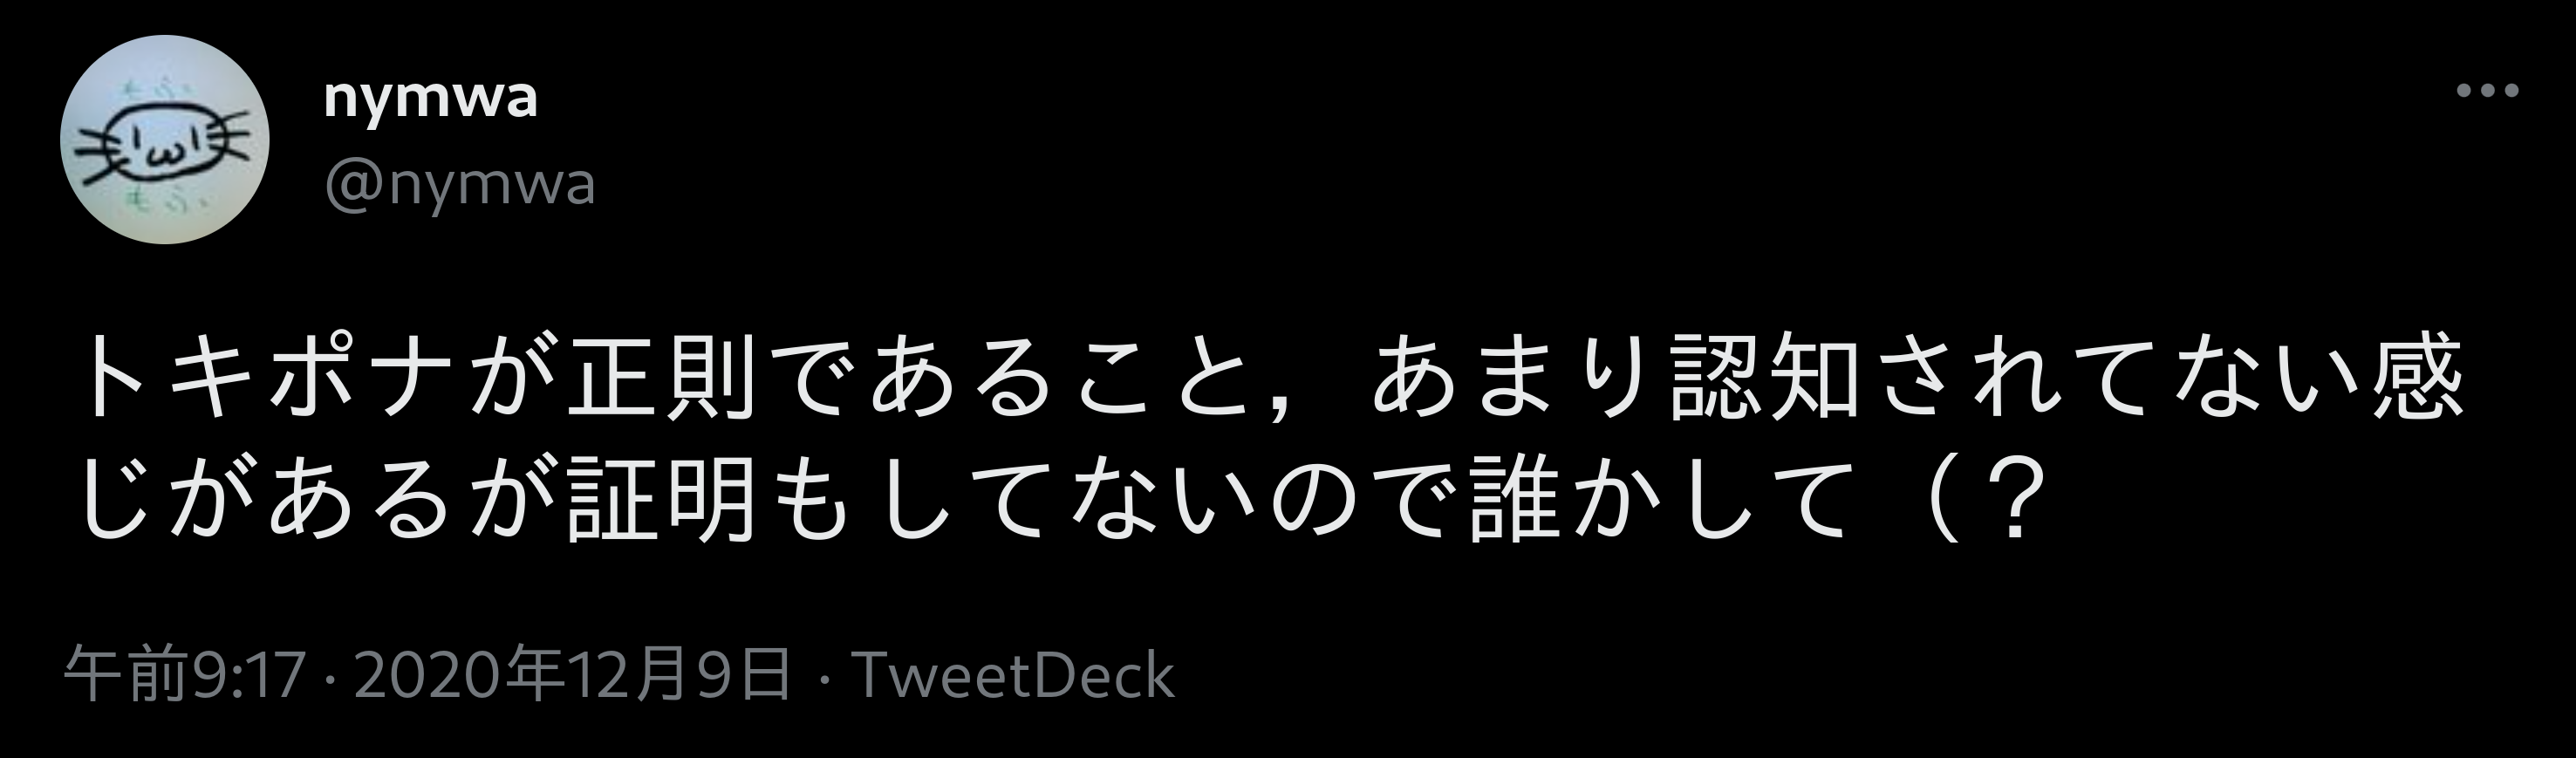
\includegraphics[width=10cm]{tweet1.png}
	\end{figure}

\end{frame}


\begin{frame}
	\frametitle{自らの正しさを信じ切る\kern.0emnymwa}

	\begin{figure}[h]
		\centering
		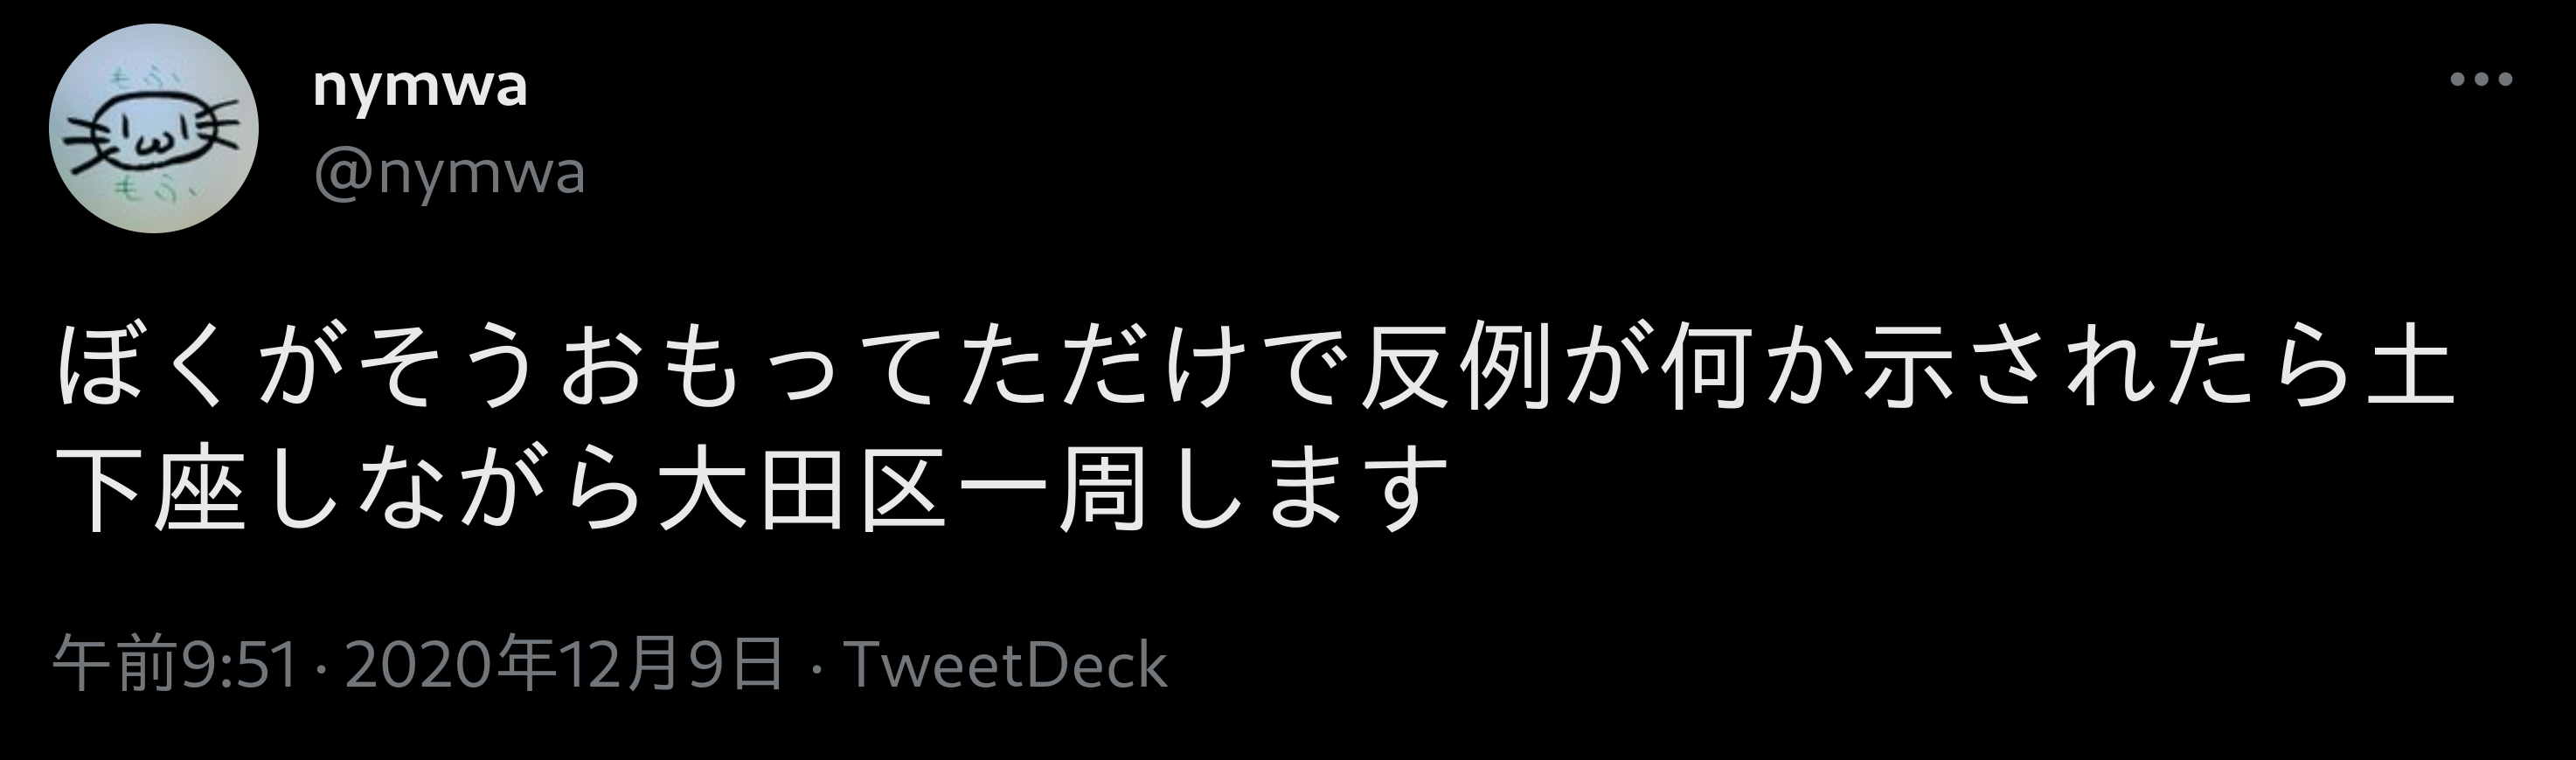
\includegraphics[width=10cm]{tweet2.png}
	\end{figure}

\end{frame}


\begin{frame}
	\frametitle{妄言の末路}

	\begin{figure}[h]
		\centering
		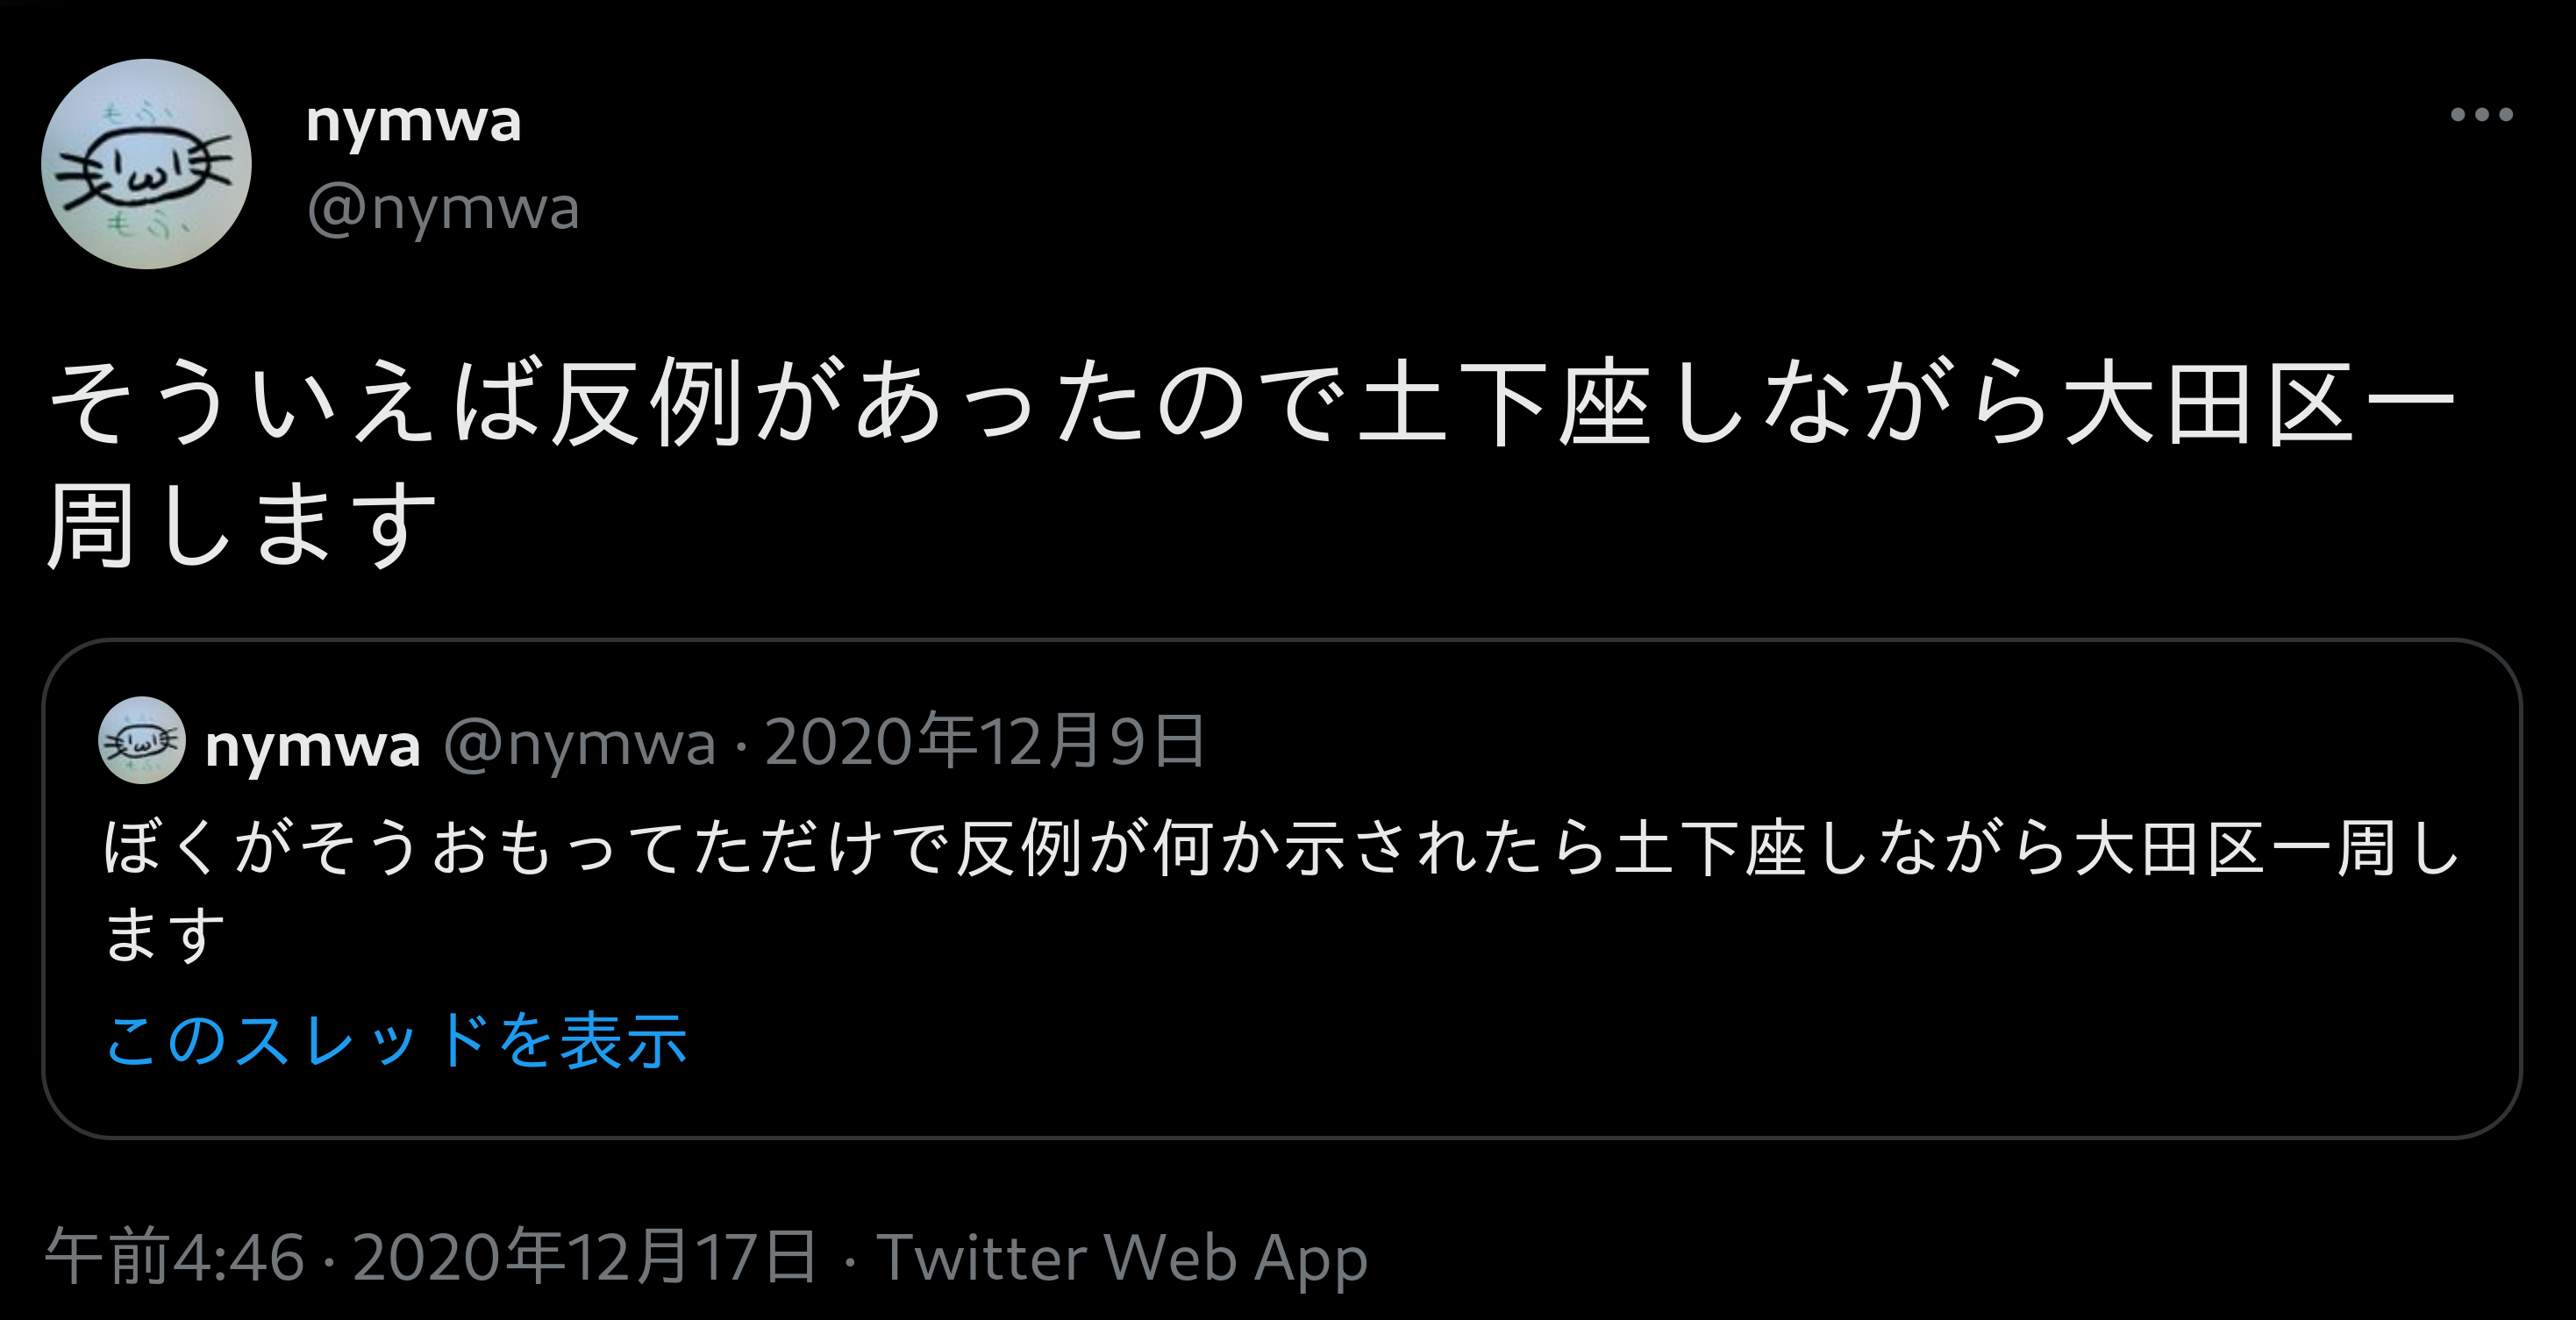
\includegraphics[width=10cm]{tweet3.png}
	\end{figure}

\end{frame}


\begin{frame}
	\frametitle{示したいこと}

	\begin{itemize}
		\item なんで私が土下座大田区一周?
		\item 以下のことを示せばいいです.
	\end{itemize}

	\begin{tcolorbox}[
			colframe=orange!80,
			colback=orange!20,
			sharp corners]
		\begin{prop}\label{prop:pona}
			トキポナは正則言語である.
		\end{prop}

		\begin{thm}
			命題\ref{prop:pona}は偽である.
		\end{thm}
	\end{tcolorbox}

\end{frame}


\begin{frame}
	\frametitle{概要}

	\begin{itemize}
		\item 次のような流れです
			\begin{itemize}
				\item 正則言語・文脈自由言語とは?
				\item トキポナは文脈自由言語でない証明
				\item トキポナは正則言語ではない!
					\begin{itemize}
						\item 文脈自由でないならば正則でもない
					\end{itemize}
			\end{itemize}
		\item 最後に土下座大田区一周の概要を説明します
	\end{itemize}

\end{frame}


\begin{frame}
	\frametitle{証明の流れ}

	\begin{itemize}
		\item コピー言語は文脈自由ではない
		\item コピー言語が文脈自由でないならば反復疑問文がある言語は文脈自由でない
		\item トキポナは反復疑問文があるため文脈自由でない
		\item トキポナは正則言語ではない
	\end{itemize}

\end{frame}


\begin{frame}
	\frametitle{形式言語}

	\begin{itemize}
		\item 言語は,単語の列の集合である.
			\begin{itemize}
				\item {\color{gray} \small 集合とは,もののあつまりのことです}
			\end{itemize}
		\item 語彙(=単語の集合)は,$\Sigma$で表します.
			\begin{itemize}
				\item 英語なら $\Sigma = \{\text{dog}, \text{cat}, \cdots\}$
				\item トキポナなら $\Sigma = \{\text{pona}, \text{ike}, \cdots\}$
				\item 2進列なら $\Sigma = \{0, 1\}$
			\end{itemize}
		\item 言語$L$は次のように定義される.
			\begin{itemize}
				\item $L = \{s | $\text{単語列}$s\text{は文法}G\text{を満たす}\}$
				\item トキポナなら $L = \{\text{toki pona li toki pona}, \cdots\}$
			\end{itemize}
	\end{itemize}
\end{frame}


\begin{frame}
	\frametitle{形式文法}

	\begin{itemize}
		\item 文法$G$は,4要素の組$(N, \Sigma, P, S)$で定義される.
			\begin{itemize}
				\item $N$: 非終端記号の(有限)集合
				\item $\Sigma$: 終端記号(=単語)の(有限)集合(=語彙)
				\item $P$: 生成規則の(有限)集合
				\item $S$: 開始記号
			\end{itemize}
		\item 「非終端記号」「終端記号」とは?
		\item 生成規則とは?
		\item 開始記号とは?
	\end{itemize}
\end{frame}


\begin{frame}
	\frametitle{非終端記号と終端記号}
\end{frame}


\begin{frame}
	\frametitle{生成規則}

	\begin{itemize}
		\item 文を生成するための規則のことです
			\begin{itemize}
				\item 非終端記号や終端記号の列を置き換えることで文を生成する!
			\end{itemize}
	\end{itemize}
\end{frame}


\begin{frame}
	\frametitle{開始記号}
\end{frame}


\begin{frame}
	\frametitle{チョムスキー階層}
\end{frame}


\begin{frame}
	\frametitle{正則言語}
\end{frame}


\begin{frame}
	\frametitle{正則言語の例}
\end{frame}


\begin{frame}
	\frametitle{文脈自由言語}
\end{frame}


\begin{frame}
	\frametitle{文脈自由言語の例}
\end{frame}


\begin{frame}
	\frametitle{文脈依存言語と句構造文法}
\end{frame}


\begin{frame}
	\frametitle{ここまで}

	\begin{itemize}
		\item 形式言語での,「言語」「文法」について説明しました
		\item 「じゃあなんでトキポナは正則言語じゃないの」
	\end{itemize}
\end{frame}


\begin{frame}
	\frametitle{なぜトキポナが正則と思ったのか?}

	\begin{itemize}
		\item トキポナはかんたん
			\begin{itemize}
				\item 再帰がない!
					\begin{itemize}
						\item I read the book I bought.
						\item mi esun e lipu. mi lukin e ona.
					\end{itemize}
			\end{itemize}
		\item 再帰がある $\Rightarrow$ 正則ではない
			\begin{itemize}
				\item 文脈自由文法は再帰を記述できる
			\end{itemize}
		\item 「トキポナは再帰がないから正則なのでは?」
			\begin{itemize}
				\item {\color{gray} \small「再帰がない $\Rightarrow$ 正則である」は真でない…}
			\end{itemize}
	\end{itemize}

\end{frame}


\begin{frame}
	\frametitle{コピー言語}
\end{frame}


\begin{frame}
	\frametitle{文脈自由言語でないことの証明とは?}
\end{frame}


\begin{frame}
	\frametitle{文脈自由言語の反復補題}
\end{frame}


\begin{frame}
	\frametitle{コピー言語は文脈自由でない}
\end{frame}


\begin{frame}
	\frametitle{コピー言語は文脈自由でない}

	\begin{center}
		\includegraphics[width=10cm]{wakannai.jpg}
	\end{center}
\end{frame}


\begin{frame}
	\frametitle{より直感的な理解}

	\begin{itemize}
		\item 交差する文脈がある
			\begin{itemize}
				\item 文脈``自由''言語は,再帰できるが交差できない
				\item 文脈依存言語は交差できる
			\end{itemize}
	\end{itemize}

	\begin{figure}[h]
		\centering
		\begin{tikzpicture}[>=latex,font=\sffamily,scale=0.9,transform shape]

			\node (a) at (0, 0) {あ};
			\node (b) at (1, 0) {い};
			\node (c) at (2, 0) {う};
			\node (d) at (3, 0) {え};
			\node (e) at (4, 0) {お};
			\node (f) at (5, 0) {あ};
			\node (g) at (6, 0) {い};
			\node (h) at (7, 0) {う};
			\node (i) at (8, 0) {え};
			\node (j) at (9, 0) {お};

			\draw[-{Latex}] (a.south) to [out=280, in=260] (f.south);
			\draw[-{Latex}] (b.south) to [out=280, in=260] (g.south);
			\draw[-{Latex}] (c.south) to [out=280, in=260] (h.south);
			\draw[-{Latex}] (d.south) to [out=280, in=260] (i.south);
			\draw[-{Latex}] (e.south) to [out=280, in=260] (j.south);

		\end{tikzpicture}
	\end{figure}

\end{frame}



\begin{frame}
	\frametitle{コピー言語は文脈依存}

	\begin{itemize}
		\item 実際に文法を定義できます.
	\end{itemize}
\end{frame}


\begin{frame}
	\frametitle{反復疑問は文脈依存}
\end{frame}


\begin{frame}
	\frametitle{トキポナは文脈依存}
\end{frame}


\begin{frame}
	\frametitle{トキポナは弱文脈依存文法}
\end{frame}


\begin{frame}
	\frametitle{トキポナは正則でないため…}
\end{frame}


\begin{frame}
	\frametitle{土下座大田区一周の概要}

	\begin{itemize}
		\item 多摩川 - 羽田 区間
			\begin{itemize}
				\item ゴムボートで土下座川下り
			\end{itemize}
		\item 天空橋 - 天王洲アイル 区間
			\begin{itemize}
				\item 土下座モノレール
			\end{itemize}
		\item 品川 - 目黒 区間
			\begin{itemize}
				\item 土下座山手線
			\end{itemize}
		\item 目黒 - 多摩川 区間
			\begin{itemize}
				\item 土下座目黒線
			\end{itemize}
		\item 乗り換えで歩くのは許してほしい
	\end{itemize}
\end{frame}


\begin{frame}
	\begin{center}
		{\Huge \liberation \color{cyan} \text{≡>ω<≡}}
	\end{center}
\end{frame}

\end{document}

